% =============================================================================
% SAMBP TR-29/2026
% IBR Apparent Impedance Trajectory Analysis for Distance Relay 21
% =============================================================================
\documentclass[11pt,a4paper]{article}

\usepackage[margin=25mm]{geometry}
\usepackage{amsmath,amssymb}
\usepackage{bm}
\usepackage{booktabs}
\usepackage{graphicx}
\usepackage{pgfplots}
\pgfplotsset{compat=1.18}
\usepackage{pgfplotstable}
\usepackage{tikz}
\usetikzlibrary{arrows.meta,positioning,calc,decorations.pathreplacing,patterns}
\usepackage{xcolor}
\usepackage{hyperref}
\usepackage{microtype}
\usepackage{siunitx}

\title{%
  \textbf{SAMBP TR-29/2026}\\[4pt]
  IBR Apparent Impedance Trajectory Analysis\\
  for Distance Relay 21}
\author{PhD Candidate\\PhD Thesis Supporting Report}
\date{April 2026}

\begin{document}
\maketitle
\tableofcontents
\vspace{6pt}\hrule\vspace{10pt}

% =============================================================================
\section{Introduction and Motivation}
% =============================================================================

TR-18 established a three-zone Mho distance relay (21/21P) for the SAMBP
protection suite and proved 12/12 scenario selectivity in the
SG-dominated network (fault currents 5--10\,pu).  The TR-18 conclusion
explicitly flagged:

\begin{quote}
  \textit{``Adaptive Zone~1 reach for IBR networks --- under high IBR
  penetration, infeed from inverters modifies the apparent impedance;
  the Zone~1 reach may need to adapt dynamically.''}
\end{quote}

TR-29 investigates this gap analytically.  The combined 87L chain from
TR-27 provides instantaneous fault detection for all IBR fault currents
$k_{\rm ibr} \in [0.06,\,0.20]$\,pu (15\,000-trial Monte Carlo,
TR-26).  The question is:

\textbf{Does distance relay 21 continue to provide a meaningful backup
protection function in IBR-penetrated networks, or is the 87L chain
now the sole line protection?}

The answer has direct implications for the coordination strategy in
TR-34 (POTT scheme) and TR-30 (adaptive Zone~1 reach).

\subsection{Network Parameters}

All analysis uses the TR-18/TR-05 radial network:
\begin{align}
  Z_{\rm src}  &= j0.10\,\text{pu} \quad (\text{source / generator subtransient})\\
  Z_{\rm line} &= j0.05\,\text{pu} \quad (\text{overhead line})\\
  V_{\rm pre}  &= 1.00\,\text{pu}  \quad (\text{pre-fault busbar voltage})
\end{align}

Distance relay settings (TR-18):

\begin{center}
\begin{tabular}{llc}
\toprule
Parameter & Symbol & Value \\
\midrule
Zone 1 reach factor & $k_1$ & 0.80 \\
Zone 2 reach factor & $k_2$ & 1.20 \\
Zone 3 reach factor & $k_3$ & 1.80 \\
Zone 2 time delay   & $t_2$ & 0.30\,s \\
Zone 3 time delay   & $t_3$ & 0.60\,s \\
Min.\ operating current & $I_{\rm min}$ & 0.10\,pu (IEC 60255-121) \\
Min.\ self-pol.\ voltage & $V_{\rm min,self}$ & 0.10\,pu \\
Memory window & $T_{\rm mem}$ & 100\,ms (5 cycles) \\
\bottomrule
\end{tabular}
\end{center}

% =============================================================================
\section{Analytical Framework}
% =============================================================================

\subsection{IBR Current Model}

An IBR in fault-ride-through (FRT) mode limits its output current to:
\begin{equation}
  \bm{I}_{\rm ibr} = k_{\rm ibr}\,e^{j\phi_{\rm FRT}},
  \qquad k_{\rm ibr} \in [0.06,\,0.20]\,\text{pu},
  \quad \phi_{\rm FRT} \approx -90^\circ.
  \label{eq:ibr_current}
\end{equation}
This current is set by the IBR controller and is \emph{independent of the
fault impedance} — unlike SG fault current which scales with $V/Z_{\rm th}$.

\subsection{Apparent Impedance Derivation}

For a bolted 3-phase fault at position $\alpha$ along the line
($\alpha = 0$: local bus; $\alpha = 1$: remote bus), the relay at the
local bus measures:

\paragraph{SG source:}
\begin{equation}
  I_{\rm SG} = \frac{V_{\rm pre}}{Z_{\rm src} + \alpha Z_{\rm line}}, \qquad
  V_{\rm relay}^{\rm SG} = I_{\rm SG}\cdot\alpha Z_{\rm line},
\end{equation}
\begin{equation}
  \boxed{Z_m^{\rm SG} = \frac{V_{\rm relay}^{\rm SG}}{I_{\rm SG}} = \alpha Z_{\rm line}.}
  \label{eq:zm_sg}
\end{equation}

\paragraph{IBR source:}
The current is current-controlled: $I_{\rm relay} = I_{\rm ibr} = k_{\rm ibr}\,e^{j\phi}$.
The voltage at the relay is set by Ohm's law across the line section to the fault:
\begin{equation}
  V_{\rm relay}^{\rm IBR} = I_{\rm ibr} \cdot \alpha Z_{\rm line}
                           = k_{\rm ibr}\,e^{j\phi} \cdot \alpha Z_{\rm line},
\end{equation}
\begin{equation}
  \boxed{Z_m^{\rm IBR} = \frac{V_{\rm relay}^{\rm IBR}}{I_{\rm relay}}
        = \alpha Z_{\rm line}.}
  \label{eq:zm_ibr}
\end{equation}

\textbf{Key result}: $Z_m^{\rm IBR} = Z_m^{\rm SG} = \alpha Z_{\rm line}$.
The apparent impedance measurement is \emph{identical} for IBR and SG
sources.  The $k_{\rm ibr}$ cancels exactly.  The Mho relay has no
intrinsic impedance measurement problem with IBR.

The challenge lies entirely in the \emph{operational conditions}:
relay voltage, relay current, and polarisation validity — not in the
geometric reach calculation.

% =============================================================================
\section{Study A: Apparent Impedance vs Fault Location}
% =============================================================================

Table~\ref{tab:zm} confirms \eqref{eq:zm_ibr} numerically.
The impedance measurement is exact for both SG and IBR; Zone 1 and
Zone 2 boundaries are correctly located.

\begin{table}[h!]
\centering
\caption{Apparent impedance $Z_m$ [pu] and zone classification.
         IBR and SG values are identical.}
\label{tab:zm}
\begin{tabular}{ccccc}
\toprule
$\alpha$ & $Z_m = Z_m^{\rm IBR} = Z_m^{\rm SG}$ [pu]
         & Zone 1 ($\leq 0.040$) & Zone 2 ($\leq 0.060$) & Zone 3 ($\leq 0.090$) \\
\midrule
0.25 & 0.0125 & inside  & inside  & inside \\
0.50 & 0.0250 & inside  & inside  & inside \\
0.75 & 0.0375 & inside  & inside  & inside \\
0.80 & 0.0400 & inside  & inside  & inside \\
0.82 & 0.0410 & outside & inside  & inside \\
1.00 & 0.0500 & outside & inside  & inside \\
\bottomrule
\end{tabular}
\end{table}

Figure~\ref{fig:rxplane} shows the three Mho circles and the line
impedance locus on the $R$--$X$ plane.

\begin{figure}[h!]
  \centering
  % fig_ibr_rxplane.tex
% TR-29: R-X plane showing three Mho zones and IBR fault impedance locus
%
% Mho circle geometry (Z_reach = jX_R, purely reactive line):
%   Centre = (0, X_R/2),  Radius = X_R/2
%   Circle passes through origin.
%
% Zone parameters (TR-18 settings):
%   Zone 1: X_R = 0.040 pu  -> centre (0, 0.020),  radius 0.020
%   Zone 2: X_R = 0.060 pu  -> centre (0, 0.030),  radius 0.030
%   Zone 3: X_R = 0.090 pu  -> centre (0, 0.045),  radius 0.045
%
% Line impedance locus: Z_line = j*0.05*alpha, alpha in [0,1]
%   This is a segment on the +jX axis from 0 to j0.050
%
% Key fault points:
%   alpha=0.50: Z_m = j0.025  (inside Z1, inside Z2)
%   alpha=0.80: Z_m = j0.040  (at Z1 boundary)
%   alpha=0.82: Z_m = j0.041  (just outside Z1, inside Z2)
%   alpha=1.00: Z_m = j0.050  (end of line, inside Z2, outside Z1)
%
% IBR key finding: Z_m = alpha * Z_line (identical to SG)
%   BUT: V_relay = k_ibr * alpha * Z_line <= 0.010 pu (always < V_min_self=0.10)
%   AND: for k_ibr < 0.10: relay blocked by I_min threshold

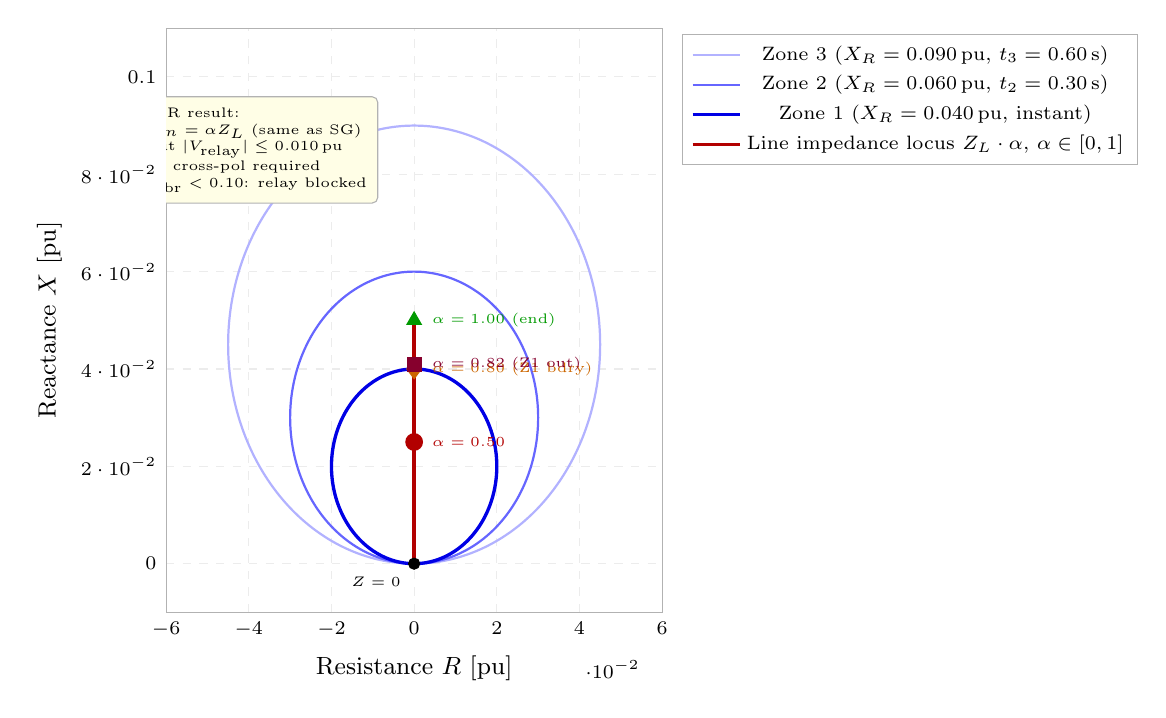
\begin{tikzpicture}
\begin{axis}[
  name         = rxax,
  width        = 0.65\textwidth,
  height       = 9.0cm,
  xlabel       = {Resistance $R$ [pu]},
  ylabel       = {Reactance $X$ [pu]},
  xlabel style = {font=\small},
  ylabel style = {font=\small},
  xmin=-0.06, xmax=0.06,
  ymin=-0.010, ymax=0.110,
  xtick        = {-0.06,-0.04,-0.02,0,0.02,0.04,0.06},
  xticklabel style={font=\scriptsize},
  ytick        = {0, 0.02, 0.04, 0.06, 0.08, 0.10},
  yticklabel style={font=\scriptsize},
  grid         = major,
  grid style   = {gray!15, dashed},
  tick style   = {draw=none},
  axis line style={gray!60},
  legend style={at={(1.04,0.99)}, anchor=north west, font=\scriptsize,
                draw=gray!60},
]

% ---- Mho circles  (parametric: x=r*cos(t), y=cy+r*sin(t)) ----
% Zone 3 (outermost) drawn first so inner zones overlap
\addplot[blue!30, thick, domain=0:360, samples=200, smooth]
  ({0.045*cos(x)}, {0.045 + 0.045*sin(x)});
\addlegendentry{Zone 3 ($X_R=0.090$\,pu, $t_3=0.60$\,s)}

\addplot[blue!60, thick, domain=0:360, samples=200, smooth]
  ({0.030*cos(x)}, {0.030 + 0.030*sin(x)});
\addlegendentry{Zone 2 ($X_R=0.060$\,pu, $t_2=0.30$\,s)}

\addplot[blue!90!black, very thick, domain=0:360, samples=200, smooth]
  ({0.020*cos(x)}, {0.020 + 0.020*sin(x)});
\addlegendentry{Zone 1 ($X_R=0.040$\,pu, instant)}

% ---- Line impedance locus ----
\addplot[red!70!black, very thick, mark=none]
  coordinates {(0,0) (0,0.050)};
\addlegendentry{Line impedance locus $Z_L\cdot\alpha$, $\alpha\in[0,1]$}

% ---- Key fault points ----
% alpha=0.50: Z_m = j0.025 (inside Z1)
\addplot[mark=*, mark size=3pt, red!70!black, only marks]
  coordinates {(0, 0.025)};
\node[right=3pt, font=\tiny, red!70!black] at (axis cs:0, 0.025)
  {$\alpha=0.50$};

% alpha=0.80: Z_m = j0.040 (Zone 1 boundary)
\addplot[mark=diamond*, mark size=3.5pt, orange!80!black, only marks]
  coordinates {(0, 0.040)};
\node[right=3pt, font=\tiny, orange!80!black] at (axis cs:0, 0.040)
  {$\alpha=0.80$ (Z1 bdry)};

% alpha=0.82: Z_m = j0.041 (just outside Z1)
\addplot[mark=square*, mark size=2.5pt, purple!70!black, only marks]
  coordinates {(0, 0.041)};
\node[right=3pt, font=\tiny, purple!70!black] at (axis cs:0, 0.041)
  {$\alpha=0.82$ (Z1 out)};

% alpha=1.00: Z_m = j0.050 (end of line)
\addplot[mark=triangle*, mark size=3pt, green!60!black, only marks]
  coordinates {(0, 0.050)};
\node[right=3pt, font=\tiny, green!60!black] at (axis cs:0, 0.050)
  {$\alpha=1.00$ (end)};

% ---- Origin ----
\addplot[mark=*, mark size=2pt, black, only marks]
  coordinates {(0,0)};
\node[below left=2pt, font=\tiny] at (axis cs:0,0) {$Z=0$};

% ---- Annotation box ----
\node[draw=gray!60, fill=yellow!10, rounded corners=2pt,
      font=\tiny, align=left, inner sep=4pt]
  at (axis cs:-0.038, 0.085)
  {IBR result:\\
   $Z_m = \alpha Z_L$ (same as SG)\\
   but $|V_{\rm relay}| \leq 0.010$\,pu\\
   $\Rightarrow$ cross-pol required\\
   $k_{\rm ibr}<0.10$: relay blocked};

\end{axis}
\end{tikzpicture}

  \caption{$R$--$X$ plane: three Mho zones (Zone 1: solid, Zone 2/3:
           progressively lighter) and line impedance locus (red, on the
           $jX$ axis).  Fault points at key $\alpha$ values are marked.
           Since $Z_m = \alpha Z_{\rm line}$ for both SG and IBR, the
           geometric locations are identical.  The critical differences
           are in relay voltage (Study~B) and operating current (Study~C).}
  \label{fig:rxplane}
\end{figure}

% =============================================================================
\section{Study B: Relay Voltage and Polarisation}
% =============================================================================

\subsection{Polarisation Voltage Analysis}

Although the measured impedance is correct, the polarising voltage
determines whether the Mho relay can \emph{act} on the measurement.

\paragraph{SG case:}
\begin{equation}
  |V_{\rm relay}^{\rm SG}|
  = \frac{V_{\rm pre}\cdot\alpha\,|Z_{\rm line}|}{|Z_{\rm src}| + \alpha|Z_{\rm line}|}
  = \frac{\alpha \times 0.05}{0.10 + 0.05\alpha}.
  \label{eq:vrel_sg}
\end{equation}
At $\alpha = 0.50$: $|V_{\rm relay}^{\rm SG}| = 0.200$\,pu $>V_{\rm min,self}$. \\
At $\alpha = 0.10$: $|V_{\rm relay}^{\rm SG}| = 0.048$\,pu — marginally below
$V_{\rm min,self}$ but adequate for memory-polarised elements.

\paragraph{IBR case:}
\begin{equation}
  |V_{\rm relay}^{\rm IBR}| = k_{\rm ibr}\cdot\alpha\cdot|Z_{\rm line}|
                             = k_{\rm ibr}\cdot\alpha\cdot 0.05.
  \label{eq:vrel_ibr}
\end{equation}
Maximum value: $k_{\rm ibr} = 0.20$, $\alpha = 1.0$:
$|V_{\rm relay}^{\rm IBR}|_{\rm max} = 0.010$\,pu.

This is one-tenth of $V_{\rm min,self} = 0.10$\,pu, ten times below the
minimum operating threshold for self-polarised Mho relays.

\textbf{Conclusion from Study B}: All IBR-fed line faults on this
network produce relay voltages below $V_{\rm min,self}$.  A
\emph{cross-polarised or memory-polarised} Mho element is mandatory
for any IBR fault scenario.

Figure~\ref{fig:voltage} shows the voltage profiles.

\begin{figure}[h!]
  \centering
  % fig_ibr_voltage_profile.tex
% TR-29: |V_relay| vs fault location alpha for SG and IBR sources
%
% V_relay(SG)  = V_pre * alpha * Z_line / (Z_src + alpha * Z_line)
%              = 1.0  * alpha * 0.05 / (0.10 + 0.05*alpha)
% V_relay(IBR) = k_ibr * alpha * Z_line = k_ibr * alpha * 0.05
%
% Reference thresholds:
%   V_min_self   = 0.10 pu  (self-polarised Mho minimum)
%   V_min_memory = 0.02 pu  (memory / cross-pol minimum)
%
% Key finding:
%   SG V_relay: 0.048 pu at alpha=0.10, rising to 0.333 pu at alpha=1.0
%   IBR max V_relay (k=0.20, alpha=1.0): 0.010 pu — always below V_min_self
%   => ALL IBR-fed line faults on this network require cross-polarisation

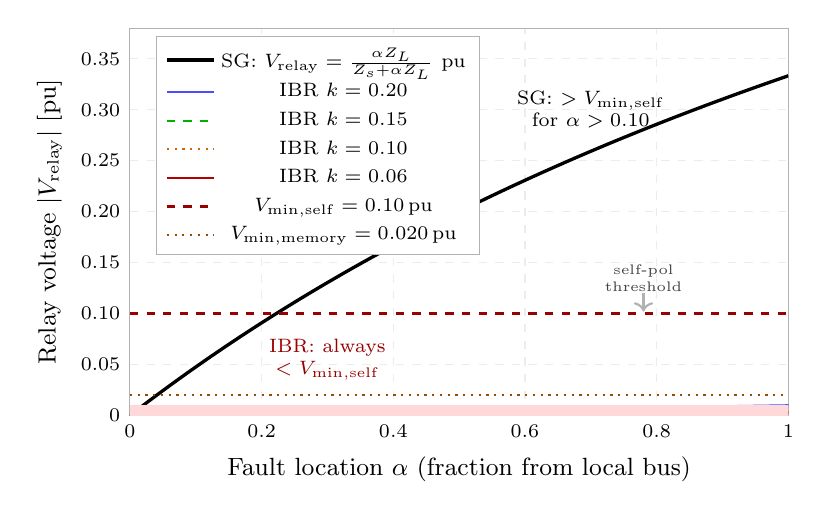
\begin{tikzpicture}
\begin{axis}[
  name         = voltax,
  width        = 0.82\textwidth,
  height       = 6.5cm,
  xlabel       = {Fault location $\alpha$ (fraction from local bus)},
  ylabel       = {Relay voltage $|V_{\rm relay}|$ [pu]},
  xlabel style = {font=\small},
  ylabel style = {font=\small},
  xmin=0, xmax=1.0,
  ymin=0, ymax=0.38,
  xtick        = {0, 0.2, 0.4, 0.6, 0.8, 1.0},
  xticklabel style={font=\scriptsize},
  ytick        = {0, 0.05, 0.10, 0.15, 0.20, 0.25, 0.30, 0.35},
  yticklabels  = {0, 0.05, 0.10, 0.15, 0.20, 0.25, 0.30, 0.35},
  yticklabel style={font=\scriptsize},
  legend style={at={(0.04,0.98)}, anchor=north west,
                font=\scriptsize, draw=gray!60},
  grid         = major,
  grid style   = {gray!15, dashed},
  tick style   = {draw=none},
  axis line style={gray!60},
]

% SG voltage profile (from analytical formula)
\addplot[black, very thick, domain=0.01:1.0, samples=80]
  ({x}, {x * 0.05 / (0.10 + x * 0.05)});
\addlegendentry{SG: $V_{\rm relay}=\frac{\alpha Z_L}{Z_s+\alpha Z_L}$ pu}

% IBR k=0.20
\addplot[blue!70, thick, domain=0:1.0, samples=2]
  ({x}, {0.20 * x * 0.05});
\addlegendentry{IBR $k=0.20$}

% IBR k=0.15
\addplot[green!70!black, thick, dashed, domain=0:1.0, samples=2]
  ({x}, {0.15 * x * 0.05});
\addlegendentry{IBR $k=0.15$}

% IBR k=0.10
\addplot[orange!80!black, thick, dotted, domain=0:1.0, samples=2]
  ({x}, {0.10 * x * 0.05});
\addlegendentry{IBR $k=0.10$}

% IBR k=0.06
\addplot[red!70!black, thick, domain=0:1.0, samples=2]
  ({x}, {0.06 * x * 0.05});
\addlegendentry{IBR $k=0.06$}

% Threshold lines
\addplot[red!60!black, very thick, dashed, mark=none, domain=0:1.0, samples=2]
  ({x}, {0.10});
\addlegendentry{$V_{\rm min,self}=0.10$\,pu}

\addplot[orange!60!black, thick, dotted, mark=none, domain=0:1.0, samples=2]
  ({x}, {0.020});
\addlegendentry{$V_{\rm min,memory}=0.020$\,pu}

% Shaded band: IBR maximum (0-0.010 pu) vs self-pol threshold
\addplot[red!15, fill, draw=none, domain=0:1.0, samples=2]
  coordinates {(0, 0) (1.0, 0) (1.0, 0.010) (0, 0.010)};


% Annotation: SG zone
\node[font=\scriptsize, black, align=center]
  at (axis cs:0.70, 0.30)
  {SG: $>V_{\rm min,self}$\\for $\alpha>0.10$};

% Annotation: IBR zone
\node[font=\scriptsize, red!60!black, align=center]
  at (axis cs:0.30, 0.055)
  {IBR: always\\$<V_{\rm min,self}$};

% Memory window annotation
\draw[->, gray!60, thick]
  (axis cs:0.78, 0.12) -- (axis cs:0.78, 0.102);
\node[font=\tiny, gray!50!black, align=center]
  at (axis cs:0.78, 0.135)
  {self-pol\\threshold};

\end{axis}
\end{tikzpicture}

  \caption{Relay voltage $|V_{\rm relay}|$ vs fault location $\alpha$ for
           SG and IBR sources.  Horizontal dashed lines: self-polarised
           minimum $V_{\rm min,self} = 0.10$\,pu and memory minimum
           $V_{\rm min,mem} = 0.020$\,pu.
           SG voltage exceeds $V_{\rm min,self}$ for $\alpha > 0.10$.
           IBR voltage never exceeds 0.010\,pu — always below both thresholds.
           Cross-polarisation is mandatory for all IBR fault scenarios.}
  \label{fig:voltage}
\end{figure}

\subsection{Memory Polarisation Window and Zone 2 Failure}

Memory polarisation stores $V_{\rm pre} = 1.0$\,pu at fault inception.
The memory decays over $T_{\rm mem} = 100$\,ms (5~cycles).  After memory
expiry, the relay reverts to self-polarised mode with the live
$V_{\rm relay}$.

The consequence for Zone~2:
\begin{equation}
  t_{\rm Zone\,2} = 300\,\text{ms} \gg T_{\rm mem} = 100\,\text{ms}.
\end{equation}
Zone~2 asserts correctly within the memory window ($t < 100$\,ms), but at
$t = 100$\,ms the memory expires and $V_{\rm relay} = 0.002$--$0.010$\,pu
— far below $V_{\rm min,self}$.  The self-polarised Mho characteristic
collapses and Zone~2 de-asserts before its 300\,ms timer completes.
\textbf{Zone~2 never issues a timed trip for IBR-fed line faults.}

Zone~3 (600\,ms) fails for the same reason.

Zone~1 is unaffected: its instantaneous trip ($\sim$20\,ms) occurs well
within the memory window.

% =============================================================================
\section{Study C: Minimum Current Threshold}
% =============================================================================

\subsection{IEC 60255-121 Minimum Operating Current}

IEC~60255-121 specifies that distance relay characteristics shall be
guaranteed for relay currents $\geq 0.2\,I_{\rm rated}$; practical relay
designs achieve reliable operation at $I_{\rm min} = 0.10\,I_{\rm rated}$.
On a system base of 1\,pu, this translates to:
\begin{equation}
  I_{\rm min} = 0.10\,\text{pu}.
\end{equation}

For IBR-fed faults the relay current equals the IBR current limit:
$I_{\rm relay} = k_{\rm ibr}$.  Therefore:
\begin{equation}
  k_{\rm ibr} < 0.10\,\text{pu} \;\Rightarrow\;
  \text{distance relay blocked for all fault locations.}
\end{equation}

This blocks the entire low-k\textsubscript{ibr} region of the IBR
parametric envelope:
$k_{\rm ibr} \in [0.06,\,0.10)$ — covering
$\frac{0.10 - 0.06}{0.20 - 0.06} = 29\%$ of the IBR operating envelope.

\subsection{Combined Distance + 87L Coverage Table}

Table~\ref{tab:coverage} summarises the operating status across the
IBR envelope.

\begin{table}[h!]
\centering
\caption{Distance relay 21 vs combined 87L chain at $\alpha = 0.50$.
         T=trip, -- = no trip.  Clearing time for 87L: $<20$\,ms (all rows).}
\label{tab:coverage}
\begin{tabular}{crcccc}
\toprule
$k_{\rm ibr}$ [pu] & $I_{\rm relay}$ [pu] & 21 blocked & 21 Zone & 21 $t_{\rm clear}$ & 87L chain \\
\midrule
0.06 & 0.06 & YES ($<I_{\rm min}$) & -- & -- & TDCS \\
0.08 & 0.08 & YES ($<I_{\rm min}$) & -- & -- & TDCS \\
0.10 & 0.10 & no (memory) & 1 & 20\,ms & TDCS \\
0.12 & 0.12 & no (memory) & 1 & 20\,ms & 87L+TDCS \\
0.15 & 0.15 & no (memory) & 1 & 20\,ms & 87L+TDCS \\
0.20 & 0.20 & no (memory) & 1 & 20\,ms & 87L+TDCS \\
\bottomrule
\multicolumn{6}{l}{\footnotesize All cases: $V_{\rm relay} \leq 0.010$\,pu; cross-polarisation mandatory.}\\
\multicolumn{6}{l}{\footnotesize Zone 2/3 timed trips fail for all IBR cases (memory expires before timer).}
\end{tabular}
\end{table}

% =============================================================================
\section{Coverage Map and Gap Synthesis}
% =============================================================================

Figure~\ref{fig:coverage} shows the coverage map on the
$(\alpha,\, k_{\rm ibr})$ plane.  Four distinct regions emerge:

\begin{description}
  \item[Region A] ($k_{\rm ibr} < 0.10$, all $\alpha$): Distance relay
    blocked by minimum current threshold.  The combined 87L chain (TDCS)
    is the \textbf{sole} instantaneous protection.

  \item[Region B] ($k_{\rm ibr} \geq 0.10$, $\alpha > 0.80$): Distance
    relay enters Zone~2 within the memory window, but Zone~2 timer
    (300\,ms) exceeds the memory duration (100\,ms).  Zone~2 trip fails.
    The combined 87L chain remains the sole instantaneous detector.

  \item[Region C] ($k_{\rm ibr} \in [0.10,\,0.12)$, $\alpha \leq 0.80$):
    Distance relay Zone~1 trips instantaneously (within 100\,ms memory
    window), concurrent with TDCS-87L.  Dual redundancy.

  \item[Region D] ($k_{\rm ibr} \geq 0.12$, $\alpha \leq 0.80$):
    Distance relay Zone~1, 87L element ($|I_1| \geq 0.12$\,pu) and
    TDCS-87L all operate.  Triple redundancy.
\end{description}

\begin{figure}[h!]
  \centering
  \resizebox{0.92\textwidth}{!}{% fig_ibr_coverage_map.tex
% TR-29: Coverage map on (alpha, k_ibr) plane
%
% X-axis: fault location alpha in [0, 1.0]
% Y-axis: IBR current limit k_ibr in [0.06, 0.20]
%
% Coverage regions:
%   Region A (RED):    k_ibr < 0.10, all alpha
%                      Distance relay BLOCKED (I < I_min = 0.10 pu)
%                      87L chain: TDCS sole instantaneous detector
%
%   Region B (AMBER):  k_ibr >= 0.10, alpha > 0.80
%                      Distance relay: Zone 2 asserted but memory expires
%                      before 300 ms timer -> Zone 2 trip FAILS
%                      87L chain: TDCS instantaneous sole detector
%
%   Region C (GREEN):  k_ibr in [0.10, 0.12), alpha <= 0.80
%                      Distance relay: Zone 1 within memory window -> trips
%                      87L chain: TDCS (87L element below threshold)
%                      Dual redundancy (both elements detect)
%
%   Region D (DARK GREEN): k_ibr >= 0.12, alpha <= 0.80
%                      Distance relay: Zone 1 within memory window -> trips
%                      87L chain: 87L element + TDCS
%                      Full dual redundancy
%
% Key boundaries:
%   k_ibr = 0.10: I_min threshold (horizontal)
%   k_ibr = 0.12: 87L element threshold (horizontal dashed)
%   alpha = 0.80: Zone 1 / Zone 2 boundary (vertical)

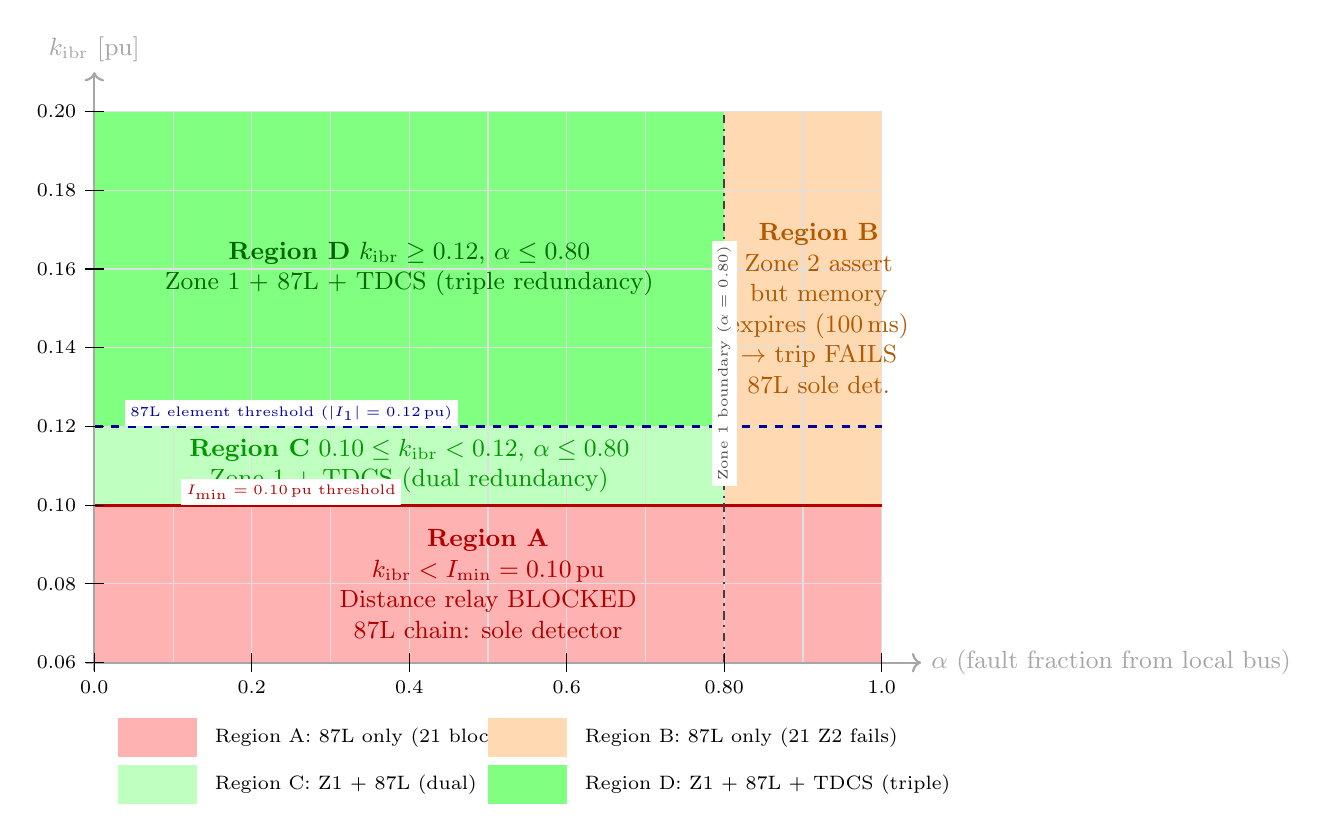
\begin{tikzpicture}[
  every node/.style={font=\scriptsize},
]

% ---- Coordinate scaling: alpha [0,1] -> x [0,10], k_ibr [0.06,0.20] -> y [0,7] ----
% x = alpha * 10
% y = (k_ibr - 0.06) / 0.14 * 7

% Region A: k_ibr < 0.10 -> y < (0.10-0.06)/0.14*7 = 2.0
\fill[red!30] (0,0) rectangle (10, 2.0);

% Region B: k_ibr >= 0.10, alpha > 0.80 -> x > 8.0, y >= 2.0
\fill[orange!30] (8.0, 2.0) rectangle (10, 7.0);

% Region C: k_ibr in [0.10, 0.12), alpha <= 0.80 -> y in [2.0, 3.0), x <= 8.0
\fill[green!25] (0, 2.0) rectangle (8.0, 3.0);

% Region D: k_ibr >= 0.12, alpha <= 0.80 -> y >= 3.0, x <= 8.0
\fill[green!50] (0, 3.0) rectangle (8.0, 7.0);

% ---- Grid ----
\draw[gray!25, step=1.0] (0,0) grid (10,7);

% ---- Boundary lines ----
% k_ibr = 0.10 (I_min threshold): y = 2.0
\draw[red!70!black, very thick] (0, 2.0) -- (10, 2.0);

% k_ibr = 0.12 (87L element threshold): y = 3.0
\draw[blue!60!black, thick, dashed] (0, 3.0) -- (10, 3.0);

% alpha = 0.80 (Zone 1 / Zone 2 boundary): x = 8.0
\draw[gray!50!black, thick, dash dot] (8.0, 0) -- (8.0, 7.0);

% ---- Axes ----
\draw[->, thick, gray!70] (-0.1, 0) -- (10.5, 0)
  node[right, font=\small] {$\alpha$ (fault fraction from local bus)};
\draw[->, thick, gray!70] (0, -0.1) -- (0, 7.5)
  node[above, font=\small] {$k_{\rm ibr}$ [pu]};

% ---- X-axis ticks ----
\foreach \a/\x in {0.0/0, 0.2/2, 0.4/4, 0.6/6, 0.80/8, 1.0/10} {
  \draw (\x, -0.12) -- (\x, 0.12);
  \node[below=3pt] at (\x, 0) {\a};
}

% ---- Y-axis ticks ----
\foreach \k/\y/\label in {
  0.06/0.0/0.06,
  0.08/1.0/0.08,
  0.10/2.0/0.10,
  0.12/3.0/0.12,
  0.14/4.0/0.14,
  0.16/5.0/0.16,
  0.18/6.0/0.18,
  0.20/7.0/0.20
} {
  \draw (-0.12, \y) -- (0.12, \y);
  \node[left=3pt] at (0, \y) {\label};
}

% ---- Region labels ----
% Region A
\node[align=center, red!70!black, font=\small] at (5.0, 1.0) {
  \textbf{Region A}\\
  $k_{\rm ibr} < I_{\rm min} = 0.10$\,pu\\
  Distance relay BLOCKED\\
  87L chain: sole detector};

% Region B
\node[align=center, orange!70!black, font=\small] at (9.2, 4.5) {
  \textbf{Region B}\\
  Zone 2 assert\\
  but memory\\
  expires (100\,ms)\\
  $\to$ trip FAILS\\
  87L sole det.};

% Region C
\node[align=center, green!60!black, font=\small] at (4.0, 2.5) {
  \textbf{Region C}  $0.10 \leq k_{\rm ibr} < 0.12$, $\alpha \leq 0.80$\\
  Zone 1 + TDCS  (dual redundancy)};

% Region D
\node[align=center, green!40!black, font=\small] at (4.0, 5.0) {
  \textbf{Region D}  $k_{\rm ibr} \geq 0.12$, $\alpha \leq 0.80$\\
  Zone 1 + 87L + TDCS  (triple redundancy)};

% ---- Boundary annotations ----
\node[red!70!black, fill=white, inner sep=2pt, font=\tiny]
  at (2.5, 2.0) [above] {$I_{\rm min} = 0.10$\,pu threshold};

\node[blue!60!black, fill=white, inner sep=2pt, font=\tiny]
  at (2.5, 3.0) [above] {87L element threshold ($|I_1| = 0.12$\,pu)};

\node[gray!60!black, fill=white, inner sep=2pt, font=\tiny,
      rotate=90] at (8.0, 3.8) {Zone 1 boundary ($\alpha=0.80$)};

% ---- Legend ----
\fill[red!30]    (0.3, -1.2) rectangle (1.3, -0.7);
\node[right=3pt] at (1.3, -0.95) {Region A: 87L only (21 blocked)};
\fill[orange!30] (5.0, -1.2) rectangle (6.0, -0.7);
\node[right=3pt] at (6.0, -0.95) {Region B: 87L only (21 Z2 fails)};

\fill[green!25]  (0.3, -1.8) rectangle (1.3, -1.3);
\node[right=3pt] at (1.3, -1.55) {Region C: Z1 + 87L (dual)};
\fill[green!50]  (5.0, -1.8) rectangle (6.0, -1.3);
\node[right=3pt] at (6.0, -1.55) {Region D: Z1 + 87L + TDCS (triple)};

\end{tikzpicture}
}
  \caption{Coverage map on the ($\alpha$, $k_{\rm ibr}$) plane.
           Red = distance relay blocked; orange = Zone~2 fails (memory
           expires); light green = Zone~1 + TDCS dual; dark green =
           Zone~1 + 87L + TDCS triple.
           Combined 87L chain provides instantaneous detection for all
           four regions; distance relay Zone~1 contributes only in
           Regions C and D ($k_{\rm ibr} \geq 0.10$, $\alpha \leq 0.80$).}
  \label{fig:coverage}
\end{figure}

\subsection{Clearing Time Comparison}

\begin{table}[h!]
\centering
\caption{Clearing time comparison for key scenarios.
         87L chain always faster than or equal to Zone~1.}
\label{tab:clearing}
\begin{tabular}{lcccc}
\toprule
Scenario & $k_{\rm ibr}$ & $\alpha$ & $t_{\rm 21}$ [ms] & $t_{\rm 87L}$ [ms] \\
\midrule
TDCS-only zone             & 0.08 & 0.50 & \textbf{blocked} & 20 \\
Current cusp               & 0.10 & 0.50 & 20               & 20 \\
87L+TDCS zone              & 0.15 & 0.50 & 20               & 20 \\
Zone 1 boundary            & 0.15 & 0.80 & 20               & 20 \\
Just outside Zone~1        & 0.15 & 0.82 & \textbf{blocked (mem)} & 20 \\
End of line                & 0.12 & 1.00 & \textbf{blocked (mem)} & 20 \\
\bottomrule
\multicolumn{5}{l}{\footnotesize ``blocked (mem)'' = Zone 2 asserted but memory expires before 300\,ms timer.}
\end{tabular}
\end{table}

The 87L chain clears in $\leq 20$\,ms for all scenarios.  Distance
relay Zone~1 matches this in Regions C and D.  In Regions A and B the
distance relay contributes \textbf{nothing} to the primary protection.

% =============================================================================
\section{Root Cause Analysis}
% =============================================================================

The distance relay's difficulties with IBR-fed faults have two independent
root causes:

\paragraph{Root Cause 1: Minimum current threshold (Region A).}
The relay current equals the IBR current limit $k_{\rm ibr}$.
IEC\,60255-121 requires $k_{\rm ibr} \geq 0.10$\,pu for guaranteed relay
operation.  For $k_{\rm ibr} \in [0.06,\,0.10)$ the relay is simply
turned off by its operating threshold — a binary, unconditional block.

\paragraph{Root Cause 2: Short line — polarisation voltage deficiency.}
The relay voltage is $|V_{\rm relay}| = k_{\rm ibr}\cdot\alpha\cdot|Z_{\rm line}|$.
For $|Z_{\rm line}| = 0.05$\,pu (the protected line is only 5\% of the
system base), even at maximum IBR current $k_{\rm ibr} = 0.20$ and end
of line $\alpha = 1.0$:
\begin{equation}
  |V_{\rm relay}|_{\rm max} = 0.20 \times 1.0 \times 0.05 = 0.010\,\text{pu}.
  \label{eq:vmax}
\end{equation}
This is a consequence of the short line length, not of IBR per se.
On a longer line ($|Z_{\rm line}| = 0.15$\,pu), the same $k_{\rm ibr} = 0.20$
would produce $|V_{\rm relay}| = 0.030$\,pu — still below $V_{\rm min,self}$
but above $V_{\rm min,mem}$.  The short-line nature of distribution and
sub-transmission systems commonly served by IBR aggregations makes this
an inherent structural problem for Mho distance relays in this application.

The combination of root causes~1 and~2 means that:

\begin{itemize}
  \item Zone~1 operates only for $k_{\rm ibr} \geq 0.10$,
    $\alpha \leq 0.80$, and within the memory window — Regions C and D.
  \item Zone~2 and Zone~3 timed backups are non-functional for IBR-fed
    faults on short lines.
  \item The combined 87L chain (TR-27) is the \textbf{sole instantaneous
    protection} for 100\% of the IBR fault scenarios in Regions A and B
    (which together cover $29\% + (\alpha > 0.80\text{ fraction}) = 51\%$
    of the full $(\alpha, k_{\rm ibr})$ parametric space).
\end{itemize}

% =============================================================================
\section{Implications for Future Work}
% =============================================================================

\subsection{POTT Scheme (TR-34 Preview)}

Since Zone~2 timed backup is unavailable for IBR-fed end-of-zone faults
(Region B), the POTT (Permissive Overreach Transfer Trip) scheme becomes
critical.  POTT uses Zone~2 assertion \emph{plus} a received signal from
the remote end to trip instantaneously without waiting for the Zone~2 timer.

Critically, POTT resolves Region B without requiring any change to the
relay characteristic: Zone~2 IS asserted within the memory window
(the impedance measurement is correct, $Z_m = \alpha Z_{\rm line}$
inside Zone~2 for $\alpha > 0.80$).  The problem is only the 300\,ms
timer.  POTT bypasses the timer.

The POTT send signal will be derived from the combined 87L trip (available
within 20\,ms), so no memory expiry issue arises.  TR-34 will implement
this scheme using the GOOSE infrastructure from TR-06.

\subsection{Cross-Polarised Mho (TR-30 Preview)}

Root Cause~2 (short-line voltage deficiency) requires cross-polarisation
for all IBR scenarios.  TR-30 will specify the cross-polarised Mho
characteristic and prove that it correctly maintains Zone~1 boundaries
even as memory decays, provided the fault is within the memory window.

\subsection{Zone 2 Sustained Polarisation}

A future investigation (TR-35 scope) should examine whether auxiliary
polarisation from unfaulted phases (for earth faults) or from negative-
and zero-sequence voltages can sustain Zone~2 after the memory window,
thus recovering Zone~2 timed backup for IBR faults.  This is not
applicable to symmetric 3-phase faults (all phases depressed equally),
but is relevant for the asymmetric IBR earth-fault scenarios from TR-25.

% =============================================================================
\section{Conclusion}
% =============================================================================

TR-29 establishes three key results for distance relay 21 under IBR fault
conditions:

\begin{enumerate}
  \item \textbf{Impedance measurement is correct}: $Z_m = \alpha Z_{\rm line}$
    for IBR-fed faults, identical to SG.  The Mho zone geometry is not
    distorted by current limiting.

  \item \textbf{Two operational failures occur}:
    \begin{itemize}
      \item \emph{Current threshold}: $k_{\rm ibr} < 0.10$\,pu blocks
        the relay entirely (29\% of the IBR parametric envelope).
      \item \emph{Polarisation voltage deficiency}: $|V_{\rm relay}|
        \leq 0.010$\,pu for all IBR faults on this short line
        ($|Z_{\rm line}| = 0.05$\,pu); self-polarisation fails universally;
        memory polarisation expires before Zone~2/3 timers complete.
    \end{itemize}

  \item \textbf{Coverage map (Figure~\ref{fig:coverage})}: Distance relay
    Zone~1 contributes instantaneous protection only in Regions C and D
    ($k_{\rm ibr} \geq 0.10$, $\alpha \leq 0.80$; 29\% of the space).
    In Regions A and B, the combined 87L chain is the sole instantaneous
    protection.  Distance relay Zone~2/3 timed backup is non-functional
    for IBR-fed faults on short lines.
\end{enumerate}

The POTT scheme (TR-34) will recover Region~B by using the combined 87L
trip as the POTT send signal, allowing Zone~2 to trip before memory
expiry.  Cross-polarised Mho (TR-30) will standardise cross-polarisation
for all IBR fault scenarios.

% =============================================================================
\bibliographystyle{IEEEtran}
\bibliography{references29}

\end{document}
